\documentclass[a4paper,5pt]{amsbook}
%%%%%%%%%%%%%%%%%%%%%%%%%%%%%%%%%%%%%%%%%%%%%%%%%%%%%%%%%%%%%%%%%%%%%

\usepackage{booktabs}
\usepackage{graphicx}
\usepackage{multicol}
\usepackage{textcomp}
\usepackage{systeme}
\usepackage{amssymb}
\usepackage[]{amsmath}
\usepackage{subcaption}
\usepackage[inline]{enumitem}
\usepackage{gensymb}

%%%%%%%%%%%%%%%%%%%%%%%%%%%%%%%%%%%%%%%%%%%%%%%%%%%%%%%%%%%%%%

\newcommand{\sen}{\,\mbox{sen}}
\newcommand{\tg}{\,\mbox{tg}\,}
\newcommand{\cosec}{\,\mbox{cosec}\,}
\newcommand{\cotg}{\,\mbox{cotg}\,}
\newcommand{\tr}{\,\mbox{tr}\,}
\newcommand{\ds}{\displaystyle}
\newcommand{\ra}{\rightarrow}

%%%%%%%%%%%%%%%%%%%%%%%%%%%%%%%%%%%%%%%%%%%%%%%%%%%%%%%%%%%%%%%%%%%%%%%%

\setlength{\textwidth}{16cm} %\setlength{\topmargin}{-1.3cm}
\setlength{\textheight}{23cm}
\setlength{\leftmargin}{1.2cm} \setlength{\rightmargin}{1.2cm}
\setlength{\oddsidemargin}{0cm}\setlength{\evensidemargin}{0cm}

%%%%%%%%%%%%%%%%%%%%%%%%%%%%%%%%%%%%%%%%%%%%%%%%%%%%%%%%%%%%%%%%%%%%%%%%

% \renewcommand{\baselinestretch}{1.6}
% \renewcommand{\thefootnote}{\fnsymbol{footnote}}
% \renewcommand{\theequation}{\thesection.\arabic{equation}}
% \setlength{\voffset}{-50pt}
% \numberwithin{equation}{chapter}

%%%%%%%%%%%%%%%%%%%%%%%%%%%%%%%%%%%%%%%%%%%%%%%%%%%%%%%%%%%%%%%%%%%%%%%

\begin{document}
\thispagestyle{empty}
\pagestyle{empty}
\begin{minipage}[h]{0.14\textwidth}
	
\includegraphics[scale=0.24]{../../ufgd.png}
\end{minipage}
\begin{minipage}[h]{\textwidth}
\begin{tabular}{c}
{{\bf UNIVERSIDADE FEDERAL DA GRANDE DOURADOS}}\\
{{\bf C\'alculo Diferencial e Integral III --- Lista 0}}\\
{{\bf Prof.\ Adriano Barbosa}}\\
\end{tabular}
\vspace{-0.45cm}
%
\end{minipage}

%------------------------

\vspace{1cm}
%%%%%%%%%%%%%%%%%%%%%%%%%%%%%%%%   formulario  inicio  %%%%%%%%%%%%%%%%%%%%%%%%%%%%%%%%
\begin{enumerate}
    \vspace{0.5cm}
    \item Para $f$ e $g$ abaixo, verifique se $f=g$.
        \begin{enumerate}
            \vspace{0.3cm}
            \item $f(x)=x+\sqrt{2-x}$ e $g(u)=u+\sqrt{2-u}$.
            \vspace{0.3cm}
            \item $f(x)=\displaystyle \frac{x^2-x}{x-1}$ e $g(x)=x$.
        \end{enumerate}

    \vspace{0.5cm}
    \item Determine se as curvas abaixo s\~ao gr\'afico de uma fun\c{c}\~ao de $x$
        \begin{figure}[h]
            \centering
            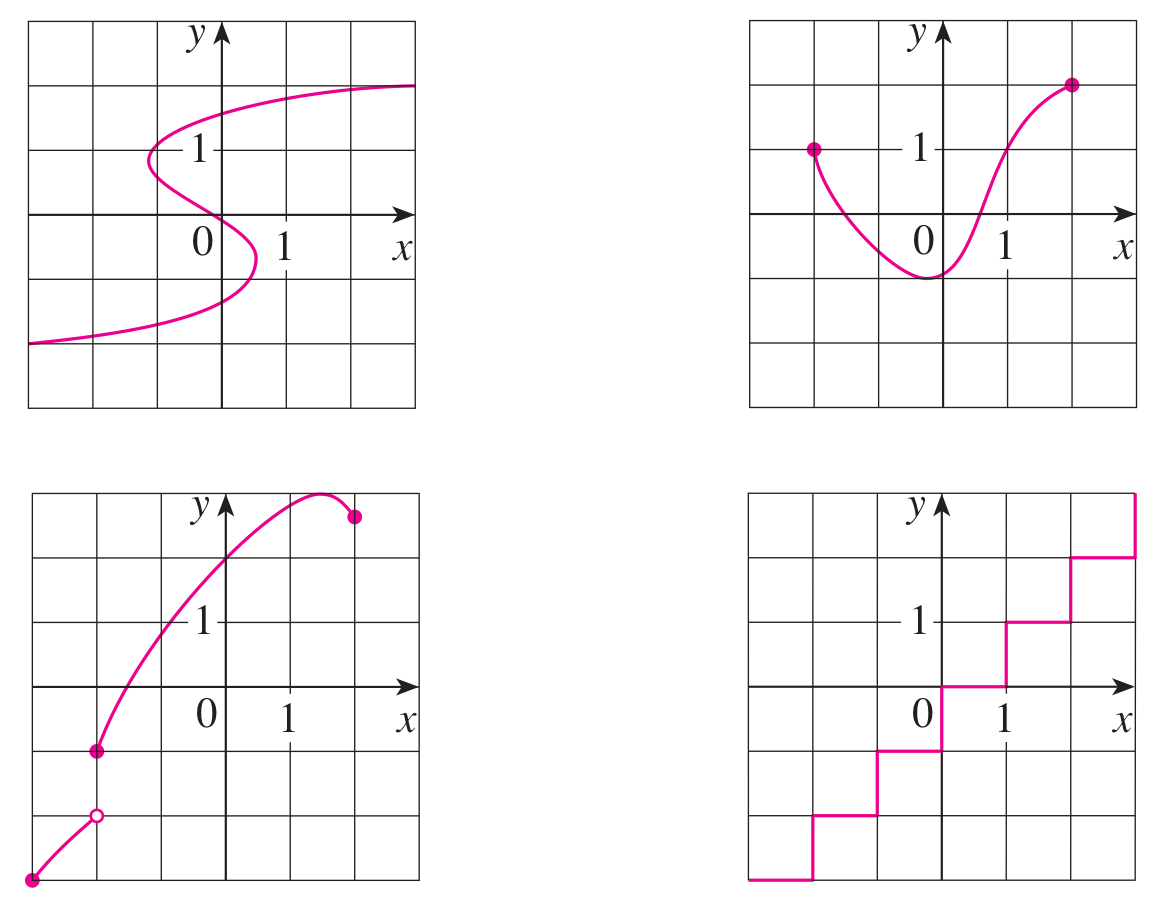
\includegraphics[width=0.5\textwidth]{lista-00-fig1.png}
        \end{figure}

    \vspace{0.5cm}
    \item Determine o maior dom\'{\i}nio das fun\c{c}\~oes abaixo:
        \begin{enumerate}
            \vspace{0.3cm}
            \item $\displaystyle f(x)=\frac{x+4}{x^2-9}$
            \vspace{0.3cm}
            \item $f(t)=\sqrt[3]{2t-1}$
            \vspace{0.3cm}
            \item $f(x)=\displaystyle\frac{2x^3-5}{x^2+x-6}$
            \vspace{0.3cm}
            \item $f(t)=\sqrt{3-t}-\sqrt{2+t}$
        \end{enumerate}

    \vspace{0.5cm}
    \item De um peda\c{c}o retangular de cartolina de dimens\~oes $8$cm$\times 15$cm,
        quatro quadrados iguais devem ser cortados, um em cada canto. A parte
        cortada remanescente \'e ent\~ao dobrada formando uma caixa aberta.
        Expresse o volume da caixa como uma fun\c{c}\~ao de $x$.

    \vspace{0.5cm}
    \item A rela\c{c}\~ao entre as escalas de temperatura Celsius (C) e Fahrenheit
        (F) \'e dada pela fun\c{c}\~ao afim $F=\displaystyle\frac{9}{5}C+32$. Desenhe o
        gr\'afico dessa fun\c{c}\~ao. Encontre o intervalo na escala F correspondente
        as temperaturas em C que est\~ao entre $18\degree$ C e $25\degree$ C.

%    \newpage
%    \vspace{0.5cm}
%    \item Para a fun\c{c}\~ao $h$ cujo gr\'afico \'e dado abaixo, determine os valores,
%        quando poss\'{\i}vel.
%
%        \begin{figure}[!h]
%            \centering
%            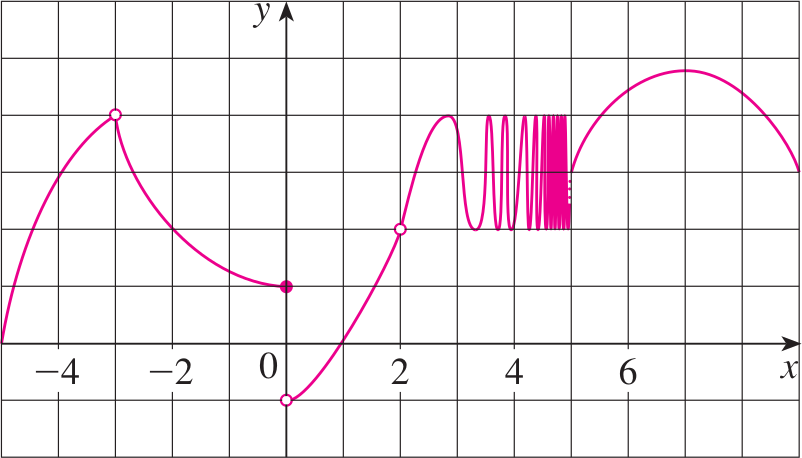
\includegraphics[width=0.5\textwidth]{lista-00-fig2.png}
%        \end{figure}
%
%        \noindent{}
%        \begin{enumerate*}
%            \item $\ds\lim_{x\ra -3^-} h(x)$
%                \hspace{0.2cm}
%                \hspace{0.2cm}
%            \item $\ds\lim_{x\ra -3^+} h(x)$
%                \hspace{0.2cm}
%                \hspace{0.2cm}
%            \item $\ds\lim_{x\ra -3} h(x)$
%                \hspace{0.2cm}
%                \hspace{0.2cm}
%            \item $h(-3)$
%                \hspace{0.2cm}
%                \hspace{0.2cm}
%            \item $\ds\lim_{x\ra 0^-} h(x)$
%                \hspace{0.2cm}
%                \hspace{0.2cm}
%            \item $\ds\lim_{x\ra 0^+} h(x)$
%                \hspace{0.2cm}
%                \hspace{0.2cm}
%            \item $\ds\lim_{x\ra 0} h(x)$
%                \hspace{0.2cm}
%                \hspace{0.2cm}
%            \item $h(0)$
%                \hspace{0.2cm}
%                \hspace{0.2cm}
%            \item $\ds\lim_{x\ra 5^-} h(x)$
%                \hspace{0.2cm}
%                \hspace{0.2cm}
%            \item $\ds\lim_{x\ra 5^+} h(x)$
%        \end{enumerate*}
%
%    \vspace{0.5cm}
%    \item Dado que $\ds\lim_{x \ra 2} f(x)=4$, $\ds\lim_{x \ra 2} g(x)=-2$ e
%        $\ds\lim_{x \ra 2} h(x)=0$, calcule os limites abaixo, caso existam.
%
%        \noindent{}
%        \begin{enumerate*}
%            \item $\ds\lim_{x \ra 2} \left[f(x)+5g(x)\right]$
%                \hspace{0.2cm}
%                \hspace{0.2cm}
%            \item $\ds\lim_{x \ra 2} {\left[g(x)\right]}^3$
%                \hspace{0.2cm}
%                \hspace{0.2cm}
%            \item $\ds\lim_{x \ra 2} \sqrt{f(x)}$
%                \hspace{0.2cm}
%                \hspace{0.2cm}
%            \item $\ds\lim_{x \ra 2} \frac{3f(x)}{g(x)}$
%                \hspace{0.2cm}
%                \hspace{0.2cm}
%            \item $\ds\lim_{x \ra 2} \frac{g(x)}{h(x)}$
%                \hspace{0.2cm}
%                \hspace{0.2cm}
%            \item $\ds\lim_{x \ra 2} \frac{g(x)h(x)}{f(x)}$
%        \end{enumerate*}
%
%    \vspace{0.5cm}
%    \item Determine em quais intervalos a fun\c{c}\~ao abaixo \'e cont\'{\i}nua.
%        \begin{figure}[h]
%            \centering
%            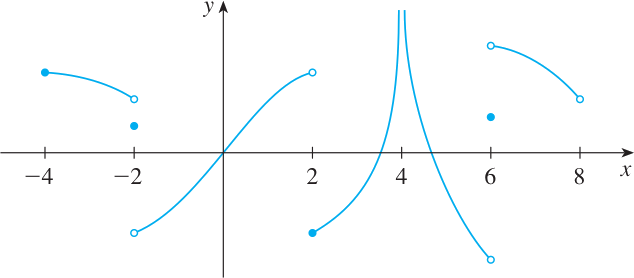
\includegraphics[width=0.5\textwidth]{lista-00-fig3.png}
%        \end{figure}
%
%    \vspace{0.5cm}
%    \item Use os teoremas sobre fun\c{c}\~oes cont\'{\i}nuas e explique porque as
%        fun\c{c}\~oes abaixo s\~ao cont\'{\i}nuas em todos os pontos do seu dom\'{\i}nio:
%        \begin{enumerate}
%            \vspace{0.3cm}
%            \item $F(x)=\ds\frac{2x^2-x-1}{x^2+1}$
%            \vspace{0.3cm}
%            \item $h(x)=\ds\frac{\sen(x)}{x+1}$
%            \vspace{0.3cm}
%            \item $g(x)=\cos(1-x^2)$
%        \end{enumerate}
%
%    \vspace{0.5cm}
%    \item Encontre a equa\c{c}\~ao da reta tangente as curvas abaixo nos pontos
%        dados:
%
%        \noindent{}
%        \begin{enumerate*}
%            \item $y=4x-3x^2$, $(2,-4)$
%            \hspace{1cm}
%            \hspace{1cm}
%            \item $y=\sqrt{x}$, $(1,1)$
%        \end{enumerate*}
%
%    \vspace{0.5cm}
%    \item O deslocamento retil\'{\i}neo de uma part\'{\i}cula \'e dado pela equa\c{c}\~ao
%        $s(t)=\ds\frac{1}{t^2}$. Determine a velocidade da part\'{\i}cula nos
%        instantes $t=1$, $t=2$ e $t=a$ com $a$ um n\'umero real positivo
%        qualquer.
%
%    \vspace{0.5cm}
%    \item Suponha $y=\sqrt{2x+1}$, onde $x$ e $y$ s\~ao fun\c{c}\~oes de $t$.  Se
%        $\ds\frac{dx}{dt}=3$, encontre $\ds\frac{dy}{dt}$ quando $x=4$.
%
%    \vspace{0.5cm}
%    \item Encontre a antiderivada mais geral para as fun\c{c}\~oes abaixo:
%        \begin{enumerate}
%            \item $f(x)=x-3$
%            \item $f(x)=\ds\frac{1}{2}+\frac{3}{4}x^2-\frac{4}{5}x^3$
%            \item $f(x)=(x+1)(2x-1)$
%            \item $f(x)=\ds\frac{1+x+x^2}{\sqrt{x}}$
%            \item $f(x)=2\sen{x}-\sec^2{x}$
%        \end{enumerate}
%
%    \vspace{0.5cm}
%    \item O gr\'afico de $g$ consiste em duas retas e um semic\'{i}rculo. Use-o
%        para calcular cada integral
%
%    \begin{enumerate*}
%    	\item $\displaystyle\int_0^2 g(x)\ dx$
%        \hspace{0.3cm}
%        \hspace{0.3cm}
%    	\item $\displaystyle\int_2^6 g(x)\ dx$
%        \hspace{0.3cm}
%        \hspace{0.3cm}
%    	\item $\displaystyle\int_0^6 g(x)\ dx$
%    \end{enumerate*}
%    
%    \begin{figure}[h]
%    	\centering
%    	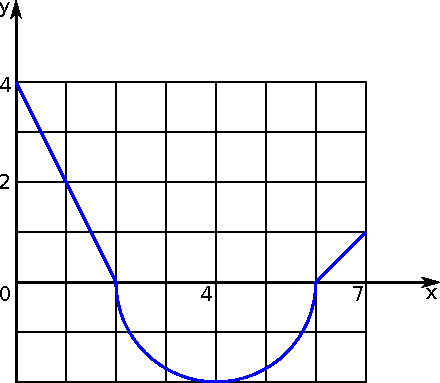
\includegraphics[scale=0.7]{lista-00-fig4.pdf}
%    \end{figure}
%    
%    \vspace{0.5cm}
%    \item Apenas analisando o gr\'afico das fun\c{c}\~oes, calcule as seguintes integrais
%
%    \begin{enumerate*}
%    	\item $\displaystyle\int_{-1}^1 x\ dx$
%        \hspace{0.1cm}
%        \hspace{0.1cm}
%    	\item $\displaystyle\int_{-1}^1 |t|\ dt$
%        \hspace{0.1cm}
%        \hspace{0.1cm}
%    	\item $\displaystyle\int_{-1}^1 y^2\ dy$
%        \hspace{0.1cm}
%        \hspace{0.1cm}
%    	\item $\displaystyle\int_{-\pi}^{\pi} \sin\theta\ d\theta$
%        \hspace{0.1cm}
%        \hspace{0.1cm}
%    	\item $\displaystyle\int_{-\pi}^{\pi} \cos\phi\ d\phi$
%    \end{enumerate*}
\end{enumerate}

\end{document}
